\documentclass[output=paper]{langsci/langscibook}
\ChapterDOI{10.5281/zenodo.573783}

\author{William A. Foley\affiliation{The University of Sydney}}
\title{Structural and semantic dependencies in word class} 
\maketitle
\begin{document}
 
\is{phrase structure} \is{lexical classes} \is{noun-verb distinction} 
\noindent Is there a dependency between the type of phrase structure that a language has and its inventory of lexical classes? This chapter will argue that there may well be, although not one that is strictly determinative. The claim is that a certain phrase structure pattern, i.e. left-headed and with overt functional categorial heads like determiners and tense-aspect-mood markers, is correlated with an attenuated distinction between nouns and verbs. A striking fact about the languages of the world is a widespread asymmetry between nouns and verbs. It is a salient but remarkable observation that languages often have many more monomorphemic nouns than they do verbs: in \ili{Yimas}, a language of New Guinea, for instance, there are over 3000 noun roots, but only around 100 verb roots, a skewing commonly found in other languages of the region \citep{Pawley1994}. Even in languages with large inventories of both classes of words, such as \ili{English}, there is a marked differential in behavior. Basic nouns in \ili{English} typically have fewer meanings and usages than verbs. The \textit{Webster’s New World College Dictionary} (\citeyear{Webster2009}), for example, lists seven meanings for the noun \textit{chair}, but no less than seventy for the verb \textit{take}. Furthermore, while the noun \textit{chair} can be used in extended meanings such as \textit{chair a meeting}, there is a clear semantic link between such uses and its basic noun meaning, while with verbs this is commonly not the case; what does \textit{take} contribute when we contrast \textit{to nap} with \textit{to take a nap}? 

\is{diachrony} \is{lexical classes!flexibility} In most language families around the world the predisposition to distinguish nouns and verbs is strong, and the distinction remains diachronically robust. But in a few, it is a family wide fact that the distinction is not so clear, and very many or most lexemes are flexible, i.e. can be freely used without clear derivational morphology either as a noun or verb. This does not mean a distinction between noun and verbs cannot be recognized; \is{noun-verb distinction} in some languages it may, and perhaps in others, it shouldn’t, but that is not my concern here. I am strictly concerned with the fact and prevalence of such flexibility and the attenuation of a sharp distinction between them. This will be looked at briefly in this chapter in the \ili{Austronesian} and \ili{Salish} language families, for which the status of the noun-verb distinction has long been controversial, and mainly concentrating on the former. What is it about the grammatical organization of \ili{Austronesian} and \ili{Salish} languages that leads to a recurring predilection to attenuate the noun-verb contrast? And as this attenuation is relatively rare crosslinguistically, what happens to this structural trait when languages bearing it come into contact with languages with the much more common property of a sharp noun-verb contrast and a different type of phrase structure? This question will be briefly looked at in areas of heavy \ili{Austronesian}-\ili{Papuan} language contact \is{language contact} in the New Guinea region.  \ili{Papuan} languages across diverse language families exhibit sharp noun-verb distinctions, even sharper than classical languages like \ili{Latin}, the source of our descriptive grammatical tradition. But it does seem that in \ili{Austronesian}-\ili{Papuan} contact situations, the selective pressures of areal features do outweigh inheritance. 

Our earliest, more sophisticated grammatical treatment of word classes goes back to the first century BC grammar of \ili{Greek} by the Alexandrian grammarian Dionysius Thrax, building on the work of Aristotle and the Stoic philosophers before him. He defined the categories of noun and verb and their distinction in the following terms:

\begin{itemize}
 \item {\textit{Ónoma} (noun): a part of speech inflected for case, signifying a person or thing} 
 \item {\textit{Rhêma} (verb): a part of speech without case inflection, but inflected for tense, person and number, signifying an activity or process performed or undergone} 
\end{itemize}

Thrax’s definitions are notable for two reasons, and both of these have influenced descriptive grammatical traditions ever since. Note that neither relies on a single criterion, both invoke two, one semantic and the other morphosyntactic. In the hothouse multicultural and multilingual atmosphere of Hellenistic Alexandria, Thrax would have been well aware of the wide differences in grammatical organization across languages, so he knew that a straightforward definition of word classes in semantic terms would not do, as items with very similar meanings could behave very differently in different languages and hence belong to different word classes. Yet he didn’t abandon semantic criteria entirely, as he was also aware of the semantic commonality of core members of each word class and the use of this as a heuristic in a first pass at identifying members of a given word class. Still, the semantic criterion on its own wouldn’t do, not only because of crosslinguistic differences, but also because the match between the typical meaning of a word class and the meanings of its individual members even in a language like \ili{Greek} wasn’t perfect; there were simply too many exceptions to what would be expected. So he dragged morphosyntactic behavior into use for delineating word class differences, for example, case for nouns and tense for verbs.

In his two pronged approach, Thrax was greatly aided by the grammatical structure of the classical languages; his description was based on \ili{Greek}. In these languages, the distinction between noun and verb is over-determined; \is{noun-verb distinction} it is virtually impossible to miss it. Consider Table \ref{tab:latin}, a map of lexical organization in terms of word class membership in \ili{Latin}.

\begin{table}
 \begin{tabular}{lcccc}
 \lsptoprule
(i) & phonology  & \textit{-a} first declension &&	  \textit{-\=e} second conjugation\\
      &           &   $\uparrow$               &&   $\uparrow$ \\                       
(ii)  & inflection &  DECLENSIONS &&  CONJUGATIONS\\
      &           &   $\uparrow$                &&   $\uparrow$ \\                       
(iii) &  syntax  & N + CASE &&  V + TENSE\\
      &           &   $\uparrow$                &&   $\uparrow$ \\                       
(iv)  & semantics  & ARGUMENT (thing) &+& PREDICATE (event)\\
\lspbottomrule
\end{tabular}
 \caption{Lexical organization in Latin}
\label{tab:latin}
\end{table}

The reason, for instance, that the noun-verb distinction was so salient to the \ili{Ancient Greek} and \ili{Latin} grammarians is the sharp differentiation in morphological behavior between them in these two languages. Not only do \ili{Ancient Greek} and \ili{Latin} have distinct grammatical categories for nouns and verbs due to their syntactic properties (level iii), e.g. case for nouns and tense for verbs, but in addition different noun and verb lexemes belong to distinct inflectional patterns (level ii), declensions for nouns and conjugations for verbs, and these in turn correlate to clear phonological contrasts in their forms (level i) (nouns belong to five phonologically contrastive declensions and verbs to four conjugations). There is overkill in the distinctiveness of these two classes in these languages; grammarians could not fail to notice it. \ili{Ancient Greek} does have word types that blend the morphosyntactic properties of nouns and verbs, such as participles, gerunds and infinitives, but these are clearly derived secondary forms and do not eclipse the very salient noun-verb distinction in these languages.

\newpage 
The classical languages with their robust distinction of word classes \is{lexical classes} have provided a largely taken for granted model for thinking about lexical distinctions ever since. Classical languages have provided us with categories of nouns, verbs and adjectives, and linguists have mainly approached language descriptions with these categories in mind (although adjectives have been more controversial) by trying to find analogs of these classical categories in the languages under description, in spite of often very different syntactic properties and inflectional categories. It is almost as if, as \citet{Riemer2010} points out, that knowing baseball and its terminology well, like first base, shortstop, home run etc., we use these familiar categories to describe all ball games: football, volleyball, tennis, basketball, etc. The real question is how much communality there is across languages that permits us to believe that we are talking about the same or even similar categories. In some languages, rather than pervasive difference as attested in \ili{Latin} and \ili{Ancient Greek}, what we find is pervasive similarity in the grammatical behavior of lexemes which are prototypically divided into these two word classes, noun and verbs, those which denote objects and those which denote events respectively. Nouns function as arguments, and verbs as predicates. \ili{St’át’imcets}, a \ili{Salish} language of British Columbia, is one such language, and as such, is typical of its language family and indeed the languages of its region \citep{DemirdacheEtAl1994}:

\ea %(1)
 use as a verb/predicate
\ea
\gll qwatsáts-kacw\\
 leave-2{\sg}.\textsc{nom}\\\jambox{\textup{event}}
\glt ‘you leave/left’
\ex 
\gll smúlhats-kacw\\ 
 woman-2{\sg}.\textsc{nom}\\\jambox{\textup{object}}
\glt ‘you are a woman’
\z
\z

\ea% { (2) 
use as noun/argument:
\ea
\gll qwatsáts-${\emptyset}$ ti smúlhats-a \\
 leave-3{\sg}.{\abs} D woman-D\\\jambox{\textup{object}}
\glt ‘the woman left’
\ex
\gll smúlhats-${\emptyset}$ ti qwatsáts-a \\
 woman-\textsc{3sg.abs} D leave-D\\\jambox{\textup{event}}
\glt ‘the leaver (one who left) is a woman’
\z
\z

\is{alignment} \is{arguments} When used as verbs, roots occur clause initially and are cliticized by a set of subject and object marking pronominals, here \textit{-(lh) kacw} for \textsc{2sg.nom} \il{St’át’imcets} (St’át’im\-cets is morphologically split ergative, so first and second person pronouns are inflected on a nominative-accusative basis, while third person exhibits an ergative absolutive pattern; third person absolutive is realized by zero, but the ergative form is \textit{–ás}). When used as nouns, the same lexemes occur in a DP headed by the determiner \textit{ti -a}; arguments are typically realized as DPs in \ili{Salish} languages. Even more striking is that lexemes of both semantic types can co-occur with such prototypical markers of verbs (going right back to Thrax’s definition more than two thousand years ago) as tense clitics like \textit{tu7} \textsc{past} and \textit{kelh} \textsc{fut}:

\ea
event\\
\ea
 \gll qwatsáts-${\emptyset}$ tu7 kw-s Gertie\\
 leave-3{\sg.\abs} \textsc{past} D-\textsc{nom} \textsc{pn}\\
 \glt ‘Gertie left’

 \ex 
 \gll qwatsáts-${\emptyset}$ kelh kw-s Gertie\\
 leave-3{\sg.\abs} {\fut} D-\textsc{nom} \textsc{pn}\\
 \glt ‘Gertie will leave’
 \z
\z

\ea
 object\\
  \ea
 \gll plísmen tu7 kw-s Bill\\
 policeman \textsc{past} D-\textsc{nom} \textsc{pn}\\
 \glt ‘Bill was a policeman’
 
  \ex
  \gll plísmen kelh kw-s Bill\\
  policeman {\fut} D-\textsc{nom} \textsc{pn} \\
  \glt ‘Bill will be a policeman’
   \z
\z

\is{noun-verb distinction} I am not claiming that no noun-verb distinction can be found in St’át’imcets and other \ili{Salish} languages. That depends on wider empirical findings and how one weighs conflicting evidence, and I do not regard this question as settled yet (see the discussion in \citeauthor{Beck2002} \citedate{Beck2002}; \citeauthor{DavisEtAl1999} \citedate{DavisEtAl1999}; \citeauthor{DemirdacheEtAl1994} \citedate{DemirdacheEtAl1994}; \citeauthor{JelinekEtAl1994} \citedate{JelinekEtAl1994}; \citeauthor{Kinkade1983} \citedate{Kinkade1983}; \citeauthor{Kuipers1968} \citedate{Kuipers1968}; \citeauthor{vanEijkEtAl1986} \citedate{vanEijkEtAl1986}). What I am simply doing here is exemplifying the pattern of flexibility in the language, and further pointing out that in the survey reported below, over 90\% of all its roots exhibited flexibility. \is{lexical classes!flexibility}

 Pretty much the same pattern is found in many \ili{Austronesian} languages and is also widespread across this vast family, although the rate is variable, as will be reported below. I illustrate here with data from \ili{Tagalog}, a language with a very high rate of flexibility: \is{lexical classes!flexibility}

 \ea%5
 use as a verb/predicate
\ea
\gll um-alis ang lalake\\
\textsc{av.perf}-leave D man\\\jambox{\textup{event}}
\glt ‘the man left’
\ex
\gll titser ang lalake\\
teacher D man \\\jambox{\textup{object}}
\glt ‘the man is a teacher’
 \z
 \z
 
\ea%6 
 use as a noun/argument:
\ea 
\gll lalake ang um-alis\\
man D \textsc{av.perf}-leave\\\jambox{\textup{event}}
\glt ‘the leaver (one who left) is a man’

\ex
\gll lalake ang titser\\
 man D teacher\\\jambox{\textup{object}}
 ‘the teacher is a man’
\z
\z

In \ili{Tagalog}, both event denoting words like \textit{umalis} ‘left’ and object denoting words like \textit{titser} ‘teacher’ function freely as arguments, the usual function of nouns and the reason for their common grammatical categories like case, by being the complements of DPs headed by a set of case marking determiners; the one illustrated in (5) and (6) is \textit{ang,} the nominative determiner. But they both are also equally good predicates, the function associated with verbs; predicates in \ili{Tagalog} are indicated by their normal initial position in the clause. Predicates are commonly specified for a number of aspectual, voice and other categories by a rich set of affixes. Crucially these are not restricted to only event denoting roots; most object denoting roots also can co-occur with them: \textit{abogado} ‘lawyer’, \textit{magabogado} ‘study to become a lawyer, engage a lawyer’; \textit{tao} ‘person’, \textit{ma-tao} ‘populated’; \textit{manok} ‘chicken’, \textit{magmanok} ‘raise chickens’; \textit{ipis} ‘cockroach’, \textit{ipis-in} ‘be infested with cockroaches’. These cannot be claimed as verbalizing suffixes because they occur also on underived verbs like \textit{mag-linis} ‘to clean’, \textit{linis-in} ‘be cleaned’, \textit{ma-nood} ‘to watch’.

\ili{St’át’imcets} and \ili{Tagalog} share a number of structural traits, and these in fact facilitate the high rate of flexibility \is{lexical classes!flexibility} in these languages. There may be other structural patterns that some languages may have hit upon to facilitate high rates of flexibility (e.g. Mundari, \citealt{EvansEtAl2005mundari}), but that found in these two languages is crosslinguistically the most common, even accounting for languages like \ili{English}. In languages like \ili{Latin} the functions of arguments and predicates, \is{arguments} \is{predicates} prototypical uses of nouns and verbs, are built into the word forms themselves, into the inflections they take. But in languages like \ili{St’át’imcets}, \ili{Tagalog} and indeed \ili{English}, this is not the case; rather these functions are indicated syntactically, not morphologically, and commonly phrasally, that is, there are phrasal functional categories like case and determiners to mark argument function and nouns and other functional categories like aspect or tense or agreement or just fixed syntactic constituent structure or perhaps a combination of these to mark predicate function and verbs. Predicate function \is{predicates} is indicated by clause initial position and by the possibility of tense or aspect inflection in \ili{St’át’imcets} and \ili{Tagalog}, and also by subject agreement clitics in the former. Argument \is{arguments} function is marked by being the complement of a determiner head in a DP in both languages (the theoretical model in which these phrase structures are cast is Lexical Functional Grammar; \citealt{Bresnan2001}; the phrase structure \is{phrase structure} \is{syntax} may look different in other frameworks and even more so in dependency based frameworks, but the basic point here about heads being functional categories would still hold):

% \begin{table}
% \begin{tabular}{lll}
%  & Predicates & Arguments\\
%  & \textbf{IP} &  \textbf{DP}\\
% \textbf{I} & (TAM) & X D X\\
% \end{tabular}
% \caption{Favored Structures for Flexible Languages.}
% \end{table}

\begin{figure}
\begin{tabular}{cp{0.2\textwidth}c}
\large {   Predicates} & { } & \large Arguments\\
&&\\
\begin{tikzpicture}
\Tree [.IP [.I{ }(TAM) ] [.X ] ]
\end{tikzpicture}
& { } & 
\begin{tikzpicture}
\Tree [.DP [.D ] [.X ] ]
\end{tikzpicture}\\
\end{tabular}
\caption{Favored structures for flexible languages}
\label{fig:favoured-structures}
\end{figure}

TAM indicates tense-aspect-mood inflection, IP indicates the projection of these inflections, and X any flexible lexeme. The phrase structure of a basic clause in both languages is identical and is shown in \figref{fig:salish}.

 
%%please move the includegraphics inside the {figure} environment

\begin{figure}
% \includegraphics[width=\textwidth]{figures/FoleyStructuralandSemanticDependenciesinWordClassMembershipREV216-img1.png}
\begin{forest}
%sn edges
[IP, for tree={parent anchor=south, child anchor=north}
  [I$'$
    [I  ]
    [S  
      [PRED ] [(DP*) ] 
    ] 
  ]
]
\end{forest}
\caption{\ili{Austronesian}/\ili{Salish} phrase structure}
\label{fig:salish}
\end{figure}

 

But there is an interesting contrast as well between \ili{St’át’imcets} and \ili{Tagalog}: the direction of derivation, \is{derivation} in other words, which of the two meanings, object denoting or event denoting corresponds to the unmarked form. In \ili{St’át’imcets} it is event denoting, while in \ili{Tagalog}, it is object denoting. Consider the data in \tabref{tab:foley:statimcetstagalog}. 


\begin{table}
\caption{Direction of Derivation in \ili{St’át’imcets} versus \ili{Tagalog} (\ili{St’át’imcets} data from \citeauthor{DavisEtAl1999} \citedate{DavisEtAl1999}). }
\label{tab:foley:statimcetstagalog}
\begin{tabularx}{\textwidth}{XX}
\lsptoprule
 \ili{St’át’imcets}  & \ili{Tagalog}\\
 \midrule
 \textit{7úqwa} ‘drink’ \newline
 \textit{s-úqwa} ‘a beverage’ & \textit{inom} ‘drinking’  \newline
			\textit{um-imom} ‘drink’\\
 \textit{núk'w7-am} ‘help’  \newline
 \textit{s-núk’wa7} ‘friend’  & \textit{tulong} ‘help’  \newline
			\textit{tulung-an} ‘help someone’\\
 \textit{cwil’-em} ‘seek’  \newline
 \textit{s-cwil’-em} ‘something sought’ & \textit{bigay} ‘gift’  \newline
			    \textit{mag-bigay} ‘give’\\

 \textit{náq’w} ‘steal’ \newline
 \textit{s-náq’w} ‘something stolen’  & \textit{nakaw} ‘something stolen’ \newline
				    \textit{mag-nakaw} ‘steal’\\
\lspbottomrule
\end{tabularx}
 \end{table}

\is{derivation} The prefix \textit{s-} in \ili{St’át’imcets} marks words which are object denoting, but in no sense can it be claimed as a derivational affix that regularly outputs nouns from basic verbs, because probably the majority of object denoting words in the language, derived or not, occur with it: \textit{skuza} ‘child’, \textit{sqáycw} ‘man’, \textit{smúlhats} ‘woman’, \textit{spzúza7} ‘bird’, \textit{sqaxwá7} ‘dog’. The point of the above examples is that in \ili{St’át’imcets}, the root form has a verb-like event denoting meaning and the noun-like object denoting meaning is derived, but in \ili{Tagalog} it is the opposite. This is most obviously brought out in the final examples of ‘steal’, ‘something stolen’.

\is{lexical classes!flexibility} But even in languages with very high rates of flexibility, it is, as we shall see, not universal, and for the classical languages like \ili{Latin}, the source of our contrasting categories of noun and verb, it is not the case that there is no flexibility (although there are certainly cases of languages with zero flexibility; this is common among the  \ili{Papuan} languages of mainland New Guinea). In \ili{Latin}, about 10\% of the lexemes of basic vocabulary in a survey I carried out with Johanna Nichols, me concentrating on \is{Pacific languages} Pacific languages, she on Eurasian and North American languages, turn out to be flexible, close to the mean crosslinguistically that we established for this feature, as in \tabref{tab:foley:calor}.

\begin{table}
%\includegraphics[width=\textwidth]{FoleyStructuralandSemanticDependenciesinWordClassMembershipREV216-img2.png} 
\caption{Flexible categorization in Latin}
\label{tab:foley:calor}
\begin{tabular}{lcccc}
 \lsptoprule
(i) & stem form & \parbox{4cm}{\centering \textit{-or} third  declension   \newline
		  \textit{\color{lsMidDarkBlue}cal\color{lsLightWine}or} `warmth'}		  &&	  \parbox{4cm}{\centering \textit{-\=e} second conjugation \newline 
						      \textit{\color{lsMidDarkBlue}cal\color{lsLightWine}\=ere} `be warm'}\\
      &           &   $\uparrow$               &&   $\uparrow$ \\                       
(ii)  & inflection &  DECLENSION &&  CONJUGATION\\
      &           &   $\uparrow$                &&   $\uparrow$ \\	                       
(iii) &  syntax  & N + CASE &&  V + TENSE\\
      &           &   $\uparrow$                &&   $\uparrow$ \\                       
(iv)  & semantics  & Subject (\textit{ónoma}) \newline 
			   &+& PREDICATE (\textit{rhêma}) \newline 
							    \\
			&&  (thing/object) & & (event)\\ 
\lspbottomrule
\end{tabular}
\end{table}
 
 
To measure rates of flexibility across languages, we drew up a list of nearly 200 basic vocabulary items and then carefully pored over grammars and dictionaries of languages to determine whether each word base was flexible or not. The list of words we used covered a wide range of semantic categories:

\begin{itemize}
\item Properties: \textit{heat, cold, length, width, dry, red, black, big, good}

\item Experiential states: \textit{fear, anger, shame, hunger, happy, sad}

\item Bodily activities: \textit{cry, sweat, sneeze, laugh, sleep, pee, poo}

\item Posture: \textit{sit, sit down, stand, stand up, lie, lie down}

\item Activities: \textit{run, walk, swim, fly, shout, sing}

\item Actions on objects: \textit{eat, bite, tear, hit, cut, open, break, throw}

\item Transfer: \textit{give, buy, say, tell}

\item Perception: \textit{see, look at, hear, listen to, know, forget}

\item Contact: \textit{pour, spill, load, empty, fill}

\item Weather: \textit{rain, thunder, lightning}

\item Body parts: \textit{ear, eye, hand, tongue, tooth, bone, elbow, hair, blood}

\item Environment: \textit{sun, moon, water, fire, sand, earth}

\item Kin: \textit{mother, father, child, sibling, spouse, name}

\item Natural kinds: \textit{dog, snake, fish, bird, pig, mouse, louse, ant, tree, leaf}

\item Artifacts: \textit{axe, spear, arrow, knife, house, broom, needle, string, clothing}

\end{itemize}

\is{lexical classes!flexibility} Flexibility was calculated as follows. A root was counted as inflexible either if 1. it had no derivational \is{derivation} processes that shifted it from being object denoting or event denoting, or 2. any derivational affix which had such a shifting function was restricted to that use only and was never used on underived forms which had the same function as the derived form. Consider the following two entries from the corpus for \ili{Tagalog}:

\begin{itemize}
\item `snake’: \textit{ahas} `snake' 
\item ‘gone’: \textit{wala} `not be, gone, extinct' \textit{mawala} `to be lost, to vanish, disappear' \textit{mawalan}, \textit{iwala} 'to lose something' \textit{ikawala} `to lose, cause one to lose something' \textit{magwala} `lose something from carelessness' \textit{makawala} `to miss, let slip by'/ `to escape' \textit{magpakawala, pakawala} `to unbind, loosen, let free' \textit{kawalan} `want, deficiency' \textit{pagkawala} `disappearance' 
\end{itemize}

\textit{ahas} ‘snake’ is not flexible because it has no possible derived forms at all, never mind those which are event denoting. Note that this would not hold for \ili{English}: \textit{the road snaked its way around the mountain;} for \ili{English} \textit{snake} would count as flexible. \textit{wala} ‘gone, disappear’ is also not flexible, because it is an event denoting predicate and all its derived forms, bar the last two, are also event denoting, predicating expressions. The only exceptions are the forms with the ``nominalizing" prefix \textit{pagka-, pagkawala} ‘disappearance’ and the circumfix \textit{ka-…-an, ka-wala-(a)n} ‘want, deficiency’, but these also fail to qualify the root for flexibility. \is{lexical classes!flexibility} The prefix \textit{pagka-} has the sole role of deriving event nominalizations and never occurs on underived object denoting words; \textit{*pagka-ahas} ‘snaking’ is impossible (the circumfix \textit{ka-…-an} is more complex, the details of which I cannot go into here; it turns out that it occurs with both object and event denoting roots, see \citealt{SchachterEtAl1972} on its functions). Now consider the following example of a flexible root in \ili{Tagalog}:

\begin{itemize}
\item ‘give’: \textit{bigay} `gift' \textit{magbigay/ibigay/bigyan} `give someone something' \textit{magbigayan} `to compromise' \textit{mamigay/ipamigay} `to distribute, give out' \textit{mapagbigayan} `to accommodate someone in providing something'
\end{itemize}

The root \textit{bigay} with no affixation at all means ‘gift’. When it takes one of the voice affixes, it then takes on the meaning ‘give’ or some other closely semantically related event type. But these voice affixes cannot be claimed to be deriving a verb from a noun root (see \citeauthor{Foley2008} \citedate{Foley2008} on this point), because voice is a necessary affixation for \textit{any} event denoting predicating word, not just those seemingly derived from object denoting ones, as the voice affixes on all the event denoting forms for \textit{wala} ‘gone’ above demonstrate. Hence \textit{bigay} counts as a flexible lexeme, used either as ‘gift’ or ‘give’ (in the latter meaning requiring, as all event denoting predicating words do, voice affixation).

 I surveyed fourteen \ili{Austronesian} languages; I report on the data from seven of them in \figref{fig:foley:fourteenlgs}:

\begin{figure} 
\caption{Rates of event/object flexibility of lexical roots between 7 \ili{Austronesian} languages}
\label{fig:foley:fourteenlgs}
     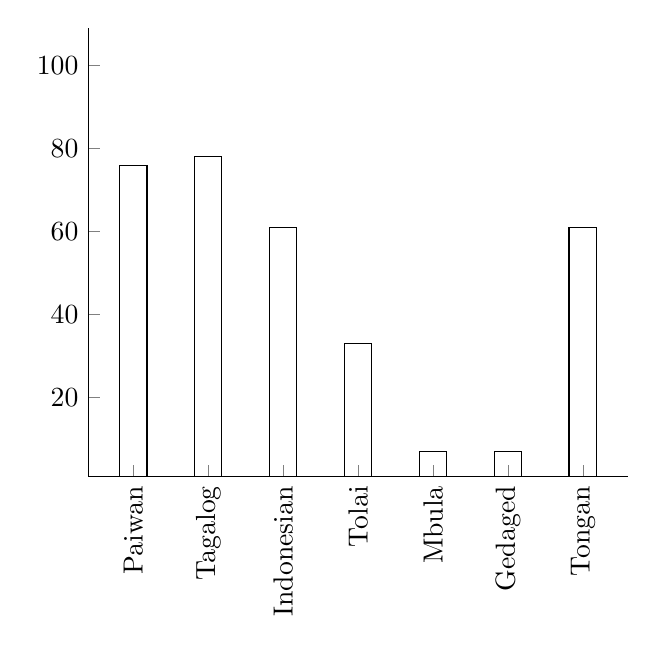
\begin{tikzpicture}
        \begin{axis}[
        	axis x line*=bottom,
            axis y line*=left,
            ymax = 100,
            ymin = 10,
            symbolic x coords = {Paiwan, Tagalog, Indonesian, Tolai, Mbula, Gedaged, Tongan},
            enlargelimits =true,
			x tick label style={rotate=90,anchor=east},
            xtick=data
          ]
            \addplot[ybar] coordinates {
                (Paiwan,   76)
                (Tagalog,  78)
                (Indonesian,   61)
                (Tolai,  33)
                (Mbula,  7)
                (Gedaged,  7)
                (Tongan,  61)
            };
        \end{axis}
    \end{tikzpicture}
\end{figure}

{\ili{Tolai}, \ili{Mbula} and \ili{Gedaged} are all New Guinea region \ili{Austronesian} languages of the \ili{Oceanic} subgroup, and all of them have lower rates of flexibility \is{lexical classes!flexibility} than their sisters further afield. But even among these three, there is a significant difference in rates of flexibility; it is much lower in \ili{Mbula} and \ili{Gedaged}, approaching nil, than in \ili{Tolai}. There are good sociolinguistic reasons for this. The contact \is{language contact} with \ili{Papuan} languages with their norm of zero flexibility has been much more intense for these two than it has been for \ili{Tolai}. So intense indeed for \ili{Gedaged} that its overall typology closely resembles its \ili{Papuan} neighbors, with verb final clausal word order, postpositions and clause chaining constructions. These data strongly support the claim that flexibility is selected \textit{against} in normal contact situations (those resulting in the genesis of pidgin and ultimately creole languages may be different). The mechanism by which language contact \is{language contact} would lead to an increase or decrease in flexibility is not at this point entirely clear; more detailed research is needed. Is it piecemeal lexeme by lexeme as they are borrowed and either adapted or adapted to, importing a flexibility \is{lexical classes!flexibility} pattern for particular lexical items and then extending that to other items at a later stage through lexical diffusion? Or is it the case that speakers of the importing language abstract a general principle of flexibility or lack thereof from the source language and apply that to different lexical roots in their own language?}
 
\largerpage
The contrastive situation between \ili{Tolai} and \ili{Tongan} is also remarkable. \ili{Tolai} and \ili{Tongan} like the other two New Guinea languages \il{Papuan} belong to the same \ili{Oceanic} subgroup of \ili{Austronesian} languages, and on archeological \is{archeology} grounds, we know that the homeland of the proto-language of this subgroup was somewhere in the Bismarck Archipelago, the region where \ili{Tolai} is spoken today. The ancestral language of \ili{Tongan} like that of \ili{Tolai}, not to mention \ili{Mbula} and \ili{Gedaged}, was spoken there. Note that the rate of flexibility of \ili{Tongan} is the same as that of \ili{Indonesian} much further to the west and generally closer to that of the languages spoken in the western region of the \ili{Austronesian} family. The languages of the west belong to a number of different high order subgroups and typically have high rates of flexibility, so on standard assumptions of historical linguistics, we would regard the high rate in \ili{Tongan} as a retention from its ancestral language. So the question arises why do we find such high retention in \ili{Tongan}, but not in \ili{Tolai}? \ili{Tolai} is in the New Guinea region, but its flexibility rate is much higher than \ili{Mbula} and \ili{Gedaged}, and its overall typology is that of a relatively conservative \ili{Oceanic} language. Its speakers are originally from New Ireland, an island where today almost exclusively \ili{Austronesian} languages are spoken. That may be the case, but there has been very significant contact with \ili{Papuan} languages in its history. The genetic data \is{genetics} tell the story. The speakers of \ili{Austronesian} languages originally migrated out of Southeast Asia, so there are certain genetic markers that are closely linked with them. Speakers of \ili{Papuan} languages, on the other hand, have been in situ in New Guinea for a very long time, at least forty thousand years, so they too are correlated with certain genetic markers. If we compare the \is{Y-chromosomal DNA} Y-chromosomal DNA, which is inherited in the male line, from the father, and mitochondrial DNA, \is{mitochondrial DNA} which passes only through the female line, from the mother, for both \ili{Tolai} and \ili{Tongan}, we find a very interesting contrast (\tabref{tab:foley:tolaitongan}, \citealt{KayserEtAl2006}).

\begin{table}
\caption{Proportion of Asian versus \ili{Papuan} Y-chromosome and mDNA markers in \ili{Tolai}-speaking and \ili{Tongan}-speaking populations}
\label{tab:foley:tolaitongan}
\begin{tabular}{lrrrr}
\lsptoprule
& \multicolumn{2}{c}{Tolai} & \multicolumn{2}{c}{Tongan}\\
                & Asian &\ili{Papuan} &Asian &   \ili{Papuan}\\
\midrule
Y-chromosome DNA & 5.3& 94.7& 41.4& 55.2\\
mitochondrial DNA &  29.4& 70.6& 92.3 &7.7\\
\lspbottomrule    
 \end{tabular}
\end{table}

\ili{Tolai} speakers have been swamped by \ili{Papuan} genes, an indication of heavy contact through interbreeding. The percentage of \ili{Papuan} Y-chromosomal DNA in \ili{Tolai} is particularly high, and this is a signal of a favored cultural pattern of \ili{Papuan} men marrying into \ili{Tolai} communities (\ili{Tolai} society like that of Proto-\ili{Oceanic} is matrilineal), though many \ili{Papuan} speaking women also contributed to the \ili{Tolai} gene pool. For \ili{Tongan} the percentages of Y-chromosomal DNA is more equally balanced, indicating that the ancestors of \ili{Tongan} speakers did interbreed with speakers of \ili{Papuan} languages   as they migrated through the New Guinea region on their way to Polynesia, but to a much lesser extent. This is to be expected, as their presence in the New Guinea region could not have lasted more than a few hundred years on current archeological evidence, while the ancestors of today’s \ili{Tolai} speakers have been there for three thousand years. But really remarkable are the percentages for mitochondrial DNA among \ili{Tongan} speakers; it is almost exclusively of Asian origin. Part of this could be due to founder effects \is{founder effects} of small populations arriving in Polynesia, but not all. What it does tell us is that very few \ili{Papuan} women entered the gene pool in the ancestral community. \ili{Papuan} men commonly interbred with \ili{Austronesian} women, but the reverse was very uncommon (again the matrilineal basis of early \ili{Oceanic} society would have had a lot to do with this). This explains the preservation of the high flexibility rate in \ili{Tongan} from Proto-\ili{Oceanic}. There is much common wisdom in the term ``mother tongue". Children were learning their language mainly from their mothers and other female relatives, and as these were \ili{Austronesian} speakers and very rarely \ili{Papuan} speakers, there was much less opportunity for the \ili{Papuan} pattern to diffuse into ancestral \ili{Tongan}.

\is{lexical classes!flexibility} Flexibility rates vary across the \ili{Austronesian} languages surveyed. And even in languages with very high rates, such as those of the Philippines and Formosa, it is never the case that flexibility is universal; some lexemes strongly resist flexibility. But this is not random. It is tied to specific semantic categories. Consider \figref{fig:foley:orangebaseline}.

\begin{sidewaysfigure}
\centering
\caption{Flexibility Rates across Semantic Types}
 \label{fig:foley:orangebaseline}
\begin{tikzpicture}
\begin{groupplot}[
    group style={
        group name=natural ontologies,
        group size=5 by 1,
        xlabels at=edge bottom,
        xticklabels at=edge bottom,
        ylabels at=edge left,
        yticklabels at=edge left,
        horizontal sep=10pt
    },
    separate axis lines,
    y axis line style={draw opacity=0},
	axis lines*=left,
	tickpos=left,
    yticklabels={\ili{Paiwan},\ili{Tagalog},\ili{Indonesian},\ili{Tolai},Tongan},
    xmin = -69,
    xmax = 69,
	ytick = data,
    width = 0.19\paperheight
%     ytick align=outside,
%     xtick align=outside
]
\nextgroupplot[title=Natural Kinds]
%natural kinds
\addplot [xbar] coordinates{
	(-45, 1)
    (-16, 2)
    (-23, 3)
    (-2, 4)
    (-25, 5)
};
\addplot[dashed] coordinates {(0,1)(0,2)(0,3)(0,4)(0,5)};
\nextgroupplot[title=Artefacts,ytick=\empty]
\addplot [xbar] coordinates{
	(18, 1)
    (5, 2)
    (39, 3)
    (34, 4)
    (0, 5)
};
\addplot[dashed] coordinates {(0,1)(0,2)(0,3)(0,4)(0,5)};
\nextgroupplot[title=Caused Events,ytick=\empty]
\addplot [xbar] coordinates{
	(-26, 1)
    (-20, 2)
    (-53, 3)
    (-17, 4)
    (-53, 5)
};
\addplot[dashed] coordinates {(0,1)(0,2)(0,3)(0,4)(0,5)};
\nextgroupplot[title=Bodily Actions,ytick=\empty]
\addplot [xbar] coordinates{
	(-19, 1)
    (22, 2)
    (3, 3)
    (3, 4)
    (-15, 5)
};
\addplot[dashed] coordinates {(0,1)(0,2)(0,3)(0,4)(0,5)};
\nextgroupplot[title=Kin Terms,ytick=\empty]
\addplot [xbar] coordinates{
	(24, 1)
    (2, 2)
    (39, 3)
    (17, 4)
    (-9, 5)
};
\addplot[dashed] coordinates {(0,1)(0,2)(0,3)(0,4)(0,5)};
\end{groupplot}
\end{tikzpicture}
\end{sidewaysfigure}

\newpage 
The central ``zero" line below each semantic category heading represents the baseline for each language, that is, the mean rate of flexibility \is{lexical classes!flexibility} across all categories for that language (\ili{Mbula} and \ili{Gedaged} are omitted from this figure because their mean is so low that nothing meaningful can be said about the distribution across categories). Under each semantic category heading, values are given for the degree to which words in that category depart from the language's baseline flexibility value. Note that certain semantic categories are mostly above the baseline, kin terms and particularly artifacts, so that they have higher flexibility rates, while others, natural kinds and especially caused actions are always below the baseline, with lower flexibility \is{lexical classes!flexibility} rates. This gives us empirical evidence for something we could call ``natural ontology". \is{natural ontology} For certain semantic categories, humans are strongly cognitively predisposed to classify the words labeling them as denoting objects or events and thereby further predisposed to only provide them with a grammatical categorization consonant with the expression of an object or an event (\citeauthor{GentnerEtAl2001}'s \citeyear{GentnerEtAl2001} cognitive dominance). In languages with a sharp noun-verb distinction \is{noun-verb distinction} this feeds directly into that grammatical and lexical distinction. But in languages not so organized, the question is more complex. What criterion do we have for saying we have a grammatical and lexical category of noun, if all clear members are restricted to denoting natural kinds? This is just erasing difference, largely due to a theoretical preference for assimilating languages to a shared base structure. I question the desirability of this move. We need to be more careful about the differences between languages before jumping to conclusions about similarities, largely on theoretical preference. If someone were to describe the difference between \ili{Latin} and languages like \ili{St’át’imcets} and \ili{Tagalog} as one ``of degree, not of kind", I would ask then empirically what would count as a difference in kind if not the data reported here? Or are our theories so poorly framed that we cannot recognize a difference in kind when we see one? Or even worse, that differences in kind simply don’t exist by virtue of theoretical fiat?



{\sloppy
\printbibliography[heading=subbibliography,notkeyword=this]
}
\end{document}%%remove this line and move all lines below to localbibliography.bib
